\chapter {Networks on Chip}
\label{Chapter.two}

Researchers have introduced Network on Chips (NoCs) in order to scale down the concepts of large scale networks to the level of System on Chips (SoCs). The communication paradigm that is used in NoCs is a packet based~\cite{Pasricha, Duato2003}, for example, 2D mesh NoC is shown in Fig.~\ref{fig:2.1}. This figure illustrates a NoC architecture with mesh topology, consisting of processing elements (\textit{PEs})  connected together with the wires through routers. In this case, a \textit{PE} (also called as \textit{node}) can be a microprocessor, an application specific integrated circuit (ASIC) block or a memory, or a combination of components connected together~\cite{Pasricha}. A \textit{network interface} (NI), present at each \textit{PE}, is used to packetize the data generated by \textit{PE}. NI is connected to a router which is responsible for routing the packets to specified destination address. There are various NoC architectures that have been proposed till date. NoC architectures can be differentiated from one another with their characteristics. Characteristics of NoCs are explained in detail in the following sections.


\begin{figure}
\vspace{10mm}
\centering
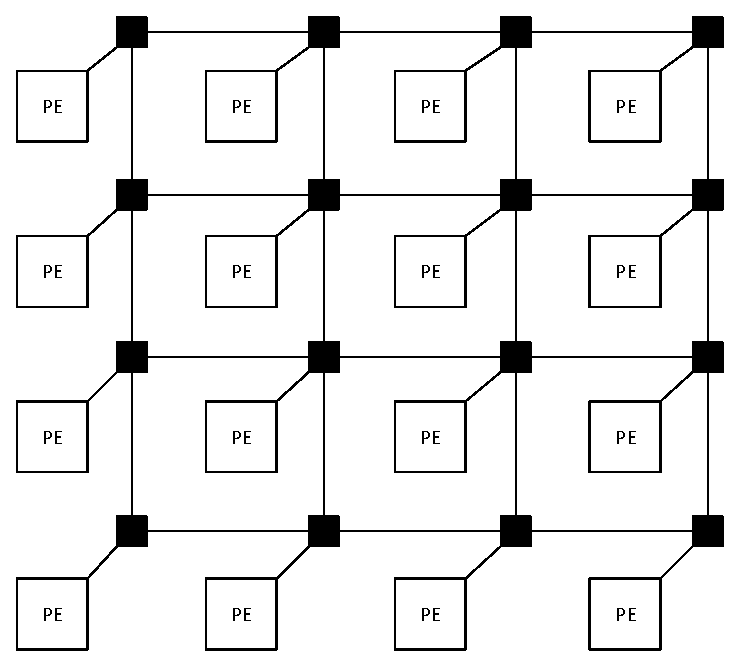
\includegraphics[height=2.8in, width=3.2in]{Mesh_topology.eps}
\caption [2D mesh NoC topology] {2D mesh NoC~\cite{Pasricha}.}
\label{fig:2.1}
\vspace{10mm}
\end{figure} 


\section{Network Topologies}

In NoC, physical organization of a interconnection network is called network topology. The topology of NoC describes how switches, nodes and links are connected to one another in a network. The NoC topologies are of three types, direct, indirect and irregular networks.

\subsection{Direct Networks}

Direct network topologies are those in which each node in the network is connected to a subset of other nodes with a direct point-to-point link. Adjacent nodes in the network are termed as \textit{neighboring} nodes. A Node can be a computational element, a memory, or a NI block which acts as router. A router is connected through links (called as channels) to the routers of the other neighboring nodes. In direct networks, when the number of nodes increases the communication bandwidth also increases. The main trade-off in the direct networks is between cost and connectivity. Performance increases with higher connectivity, but implementing router and link connection consumes more energy and results in higher area costs. It is better to avoid fully connected direct networks as shown in Fig.~\ref{fig:2.2a}, in which each node is connected directly to every other node. Hence, more common implementations of direct networks require messages to pass through several intermediate nodes before reaching the destination.


\begin{figure}
\vspace{10mm}
\centering
\begin{subfigure}{.5\textwidth}
  \centering
  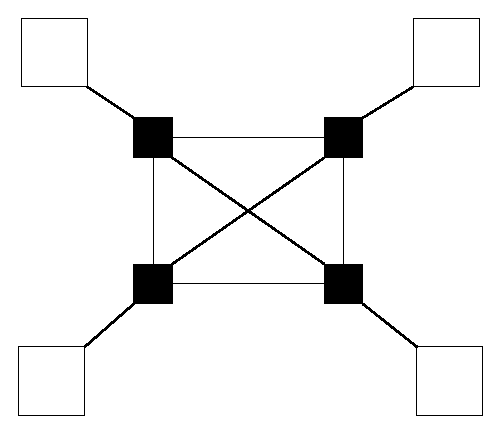
\includegraphics[width=.9\linewidth]{point_to_point.eps}
  \caption{Point-to-point network topology.}
  \label{fig:2.2a}
\end{subfigure}%
\begin{subfigure}{.5\textwidth}
  \centering
  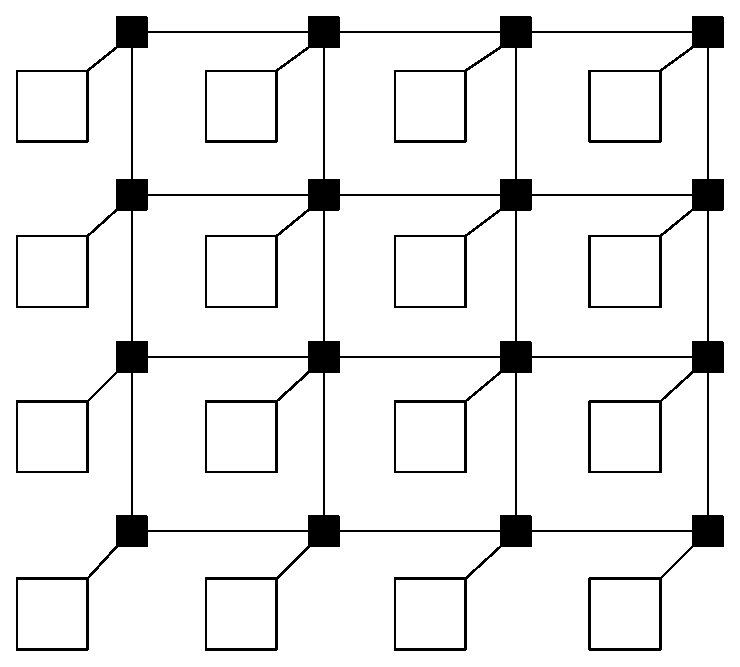
\includegraphics[width=.9\linewidth]{Mesh_topology_2.eps}
  \caption{mesh.}
  \label{fig:2.2b}
\end{subfigure}
\caption[point-to-point and mesh]{Network topologies: (a). point-to-point (b). mesh.}
\label{fig:2.2}
\vspace{10mm}
\end{figure}


Many of the direct network topologies are orthogonally implemented, meaning that nodes in the network are arranged in an n-dimensional orthogonal space and the links to the nodes produce displacement in the single direction. Routing for these networks is simple and can be efficiently implemented in hardware. There are several types of orthogonal network topologies such as n-dimensional mesh, hypercube, torus, folded torus and octagon. Mesh topology is most popularly used in NoC architectures among the above mentioned topologies. The reason for this is that its physical design is easy as all the links in the network are of same length. 

An example of a 2D mesh topology is shown in Fig.~\ref{fig:2.2b}. In this 2D network, every node is connected to four adjacent nodes other than those at the edges. We can easily add and remove the number of nodes in the network, which on the whole affects the networks area. The torus topology is also named as \textit{k}-ary \textit{n}-cube network which means a \textit{n}-dimensional grid consisting of \textit{k}-nodes in each dimension. A \textit{k}-ary 1-cube (1D torus) is a ring network which has \textit{k} nodes. An example of 4-ary 1-cube is shown in Fig.~\ref{fig:2.3a}. The main drawback of this network is its limited scalability. When the number of the nodes in the network increases, its performance decreases.  


\begin{figure}
\vspace{10mm}
\centering
\begin{subfigure}{.5\textwidth}
  \centering
  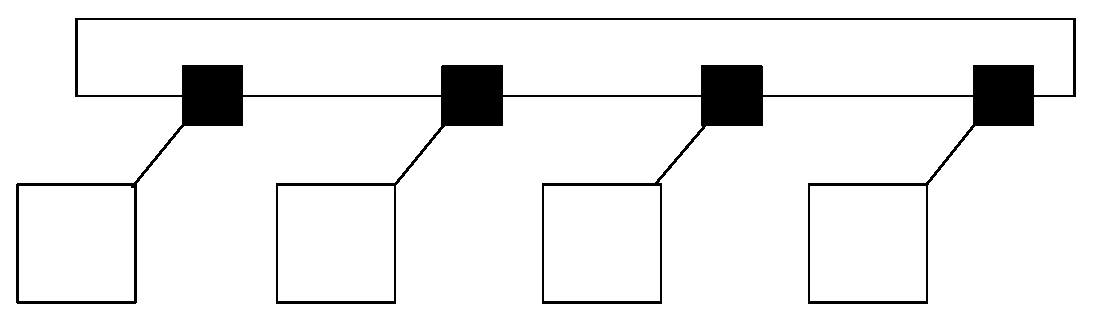
\includegraphics[width=.9\linewidth]{Ring.eps}
  \caption{Ring}
  \label{fig:2.3a}
\end{subfigure}%
\begin{subfigure}{.5\textwidth}
  \centering
  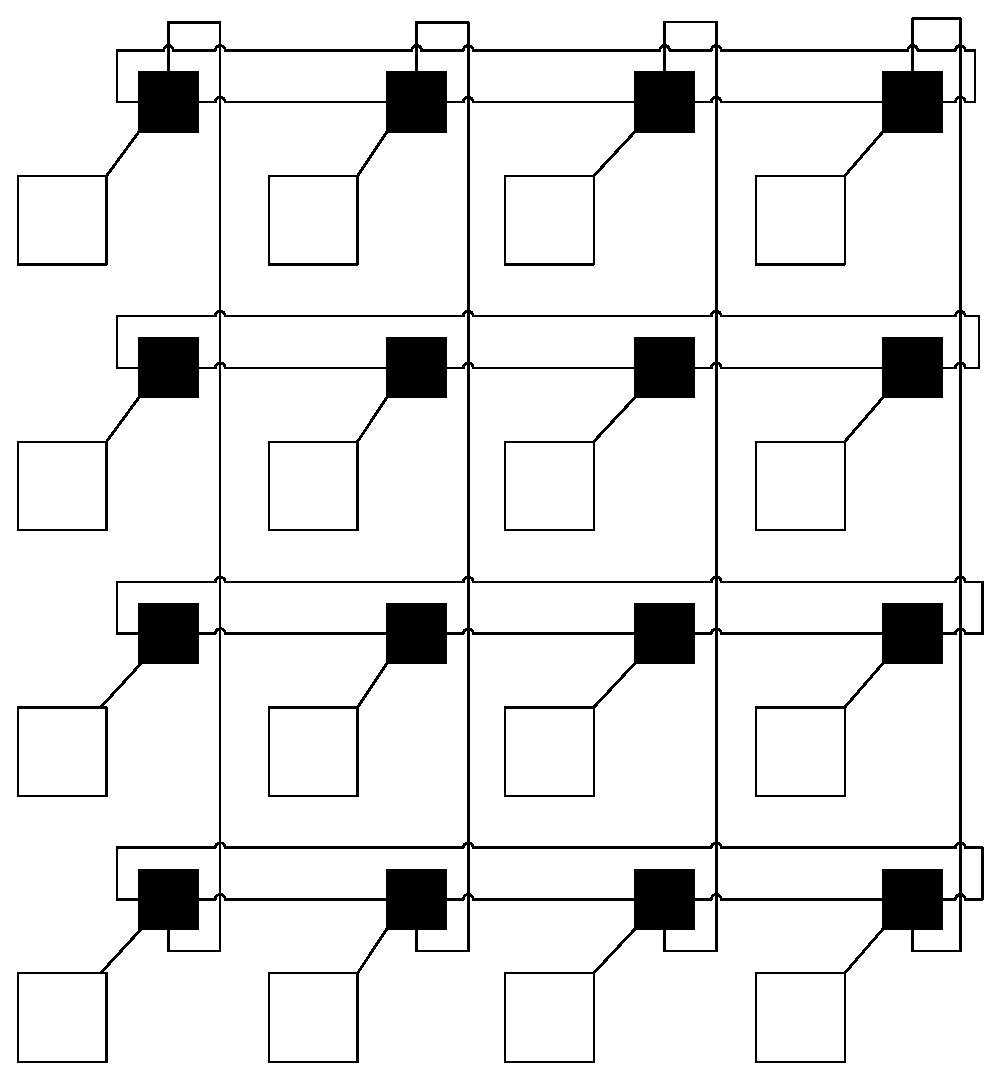
\includegraphics[width=.9\linewidth]{torus.eps}
  \caption{Torus}
  \label{fig:2.3b}
\end{subfigure}
\caption[Ring and Torus]{Network topologies (a). Ring (b). Torus.}
\label{fig:2.3}
\vspace{10mm}
\end{figure}




A 4-ary 2-cube (4x4 2D) torus is shown in Fig.~\ref{fig:2.3b}. This topology is similar to that of a 2D mesh topology except that the wrap-around channels are used to connect the nodes at the edges to the switches at the opposite edge. Each node in this network is connected to four nodes. The long connections in this network lead to delays in message transfer. This drawback is rectified by using a folding torus network topology which is shown in Fig.~\ref{fig:2.4a}. In this folded torus topology all the links have same size. A \textit{k}-ary \textit{n}-cube where \textit{k} = 2 is an \textit{n}-dimensional cube which is generally referred as a hypercube~\cite{Pasricha}. Performance can be increased, for example, by extending the torus or by adding bypass links. Adding bypass links will, however, result in higher area costs. 


\begin{figure}
\vspace{10mm}
\centering
\begin{subfigure}{.5\textwidth}
  \centering
  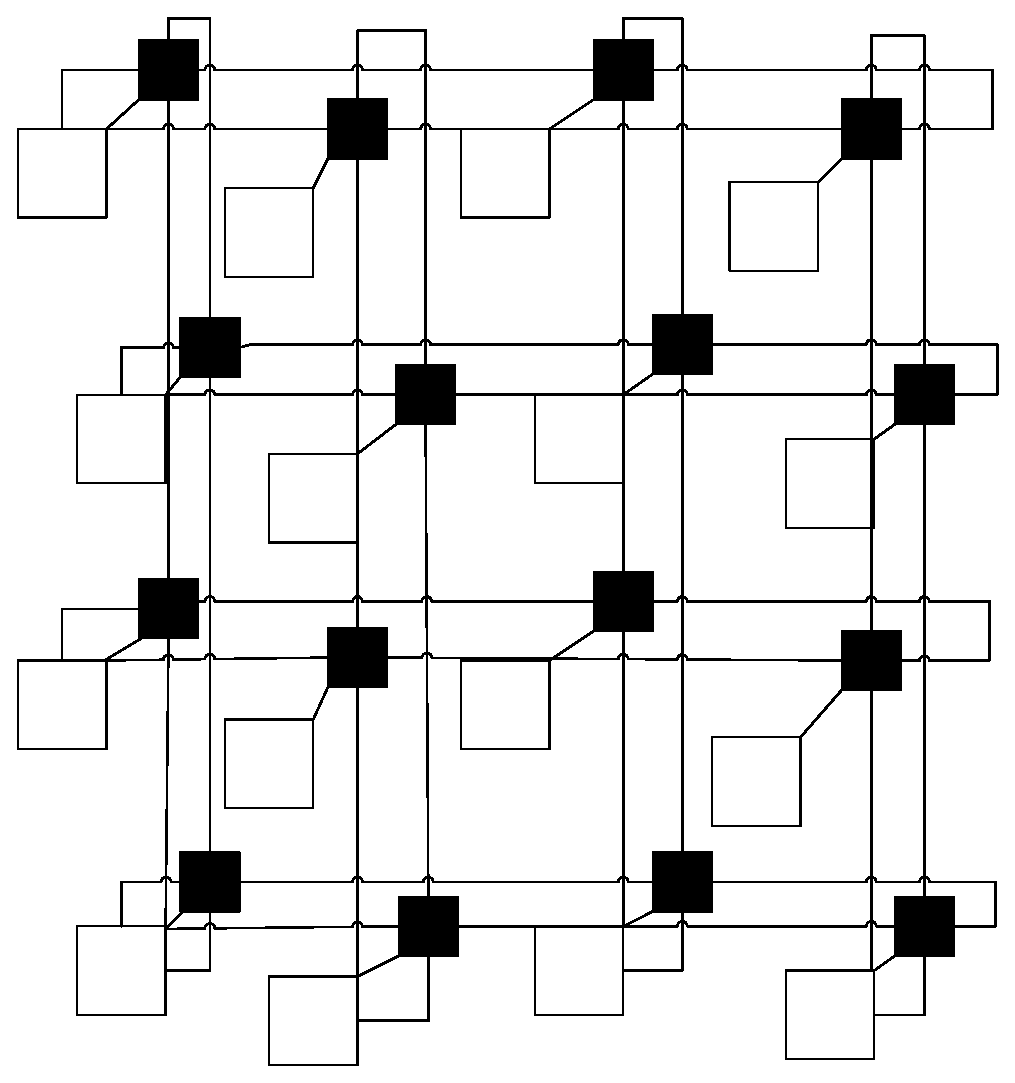
\includegraphics[width=.9\linewidth]{torusfolded.eps}
  \caption{Folded Torus}
  \label{fig:2.4a}
\end{subfigure}%
\begin{subfigure}{.5\textwidth}
  \centering
  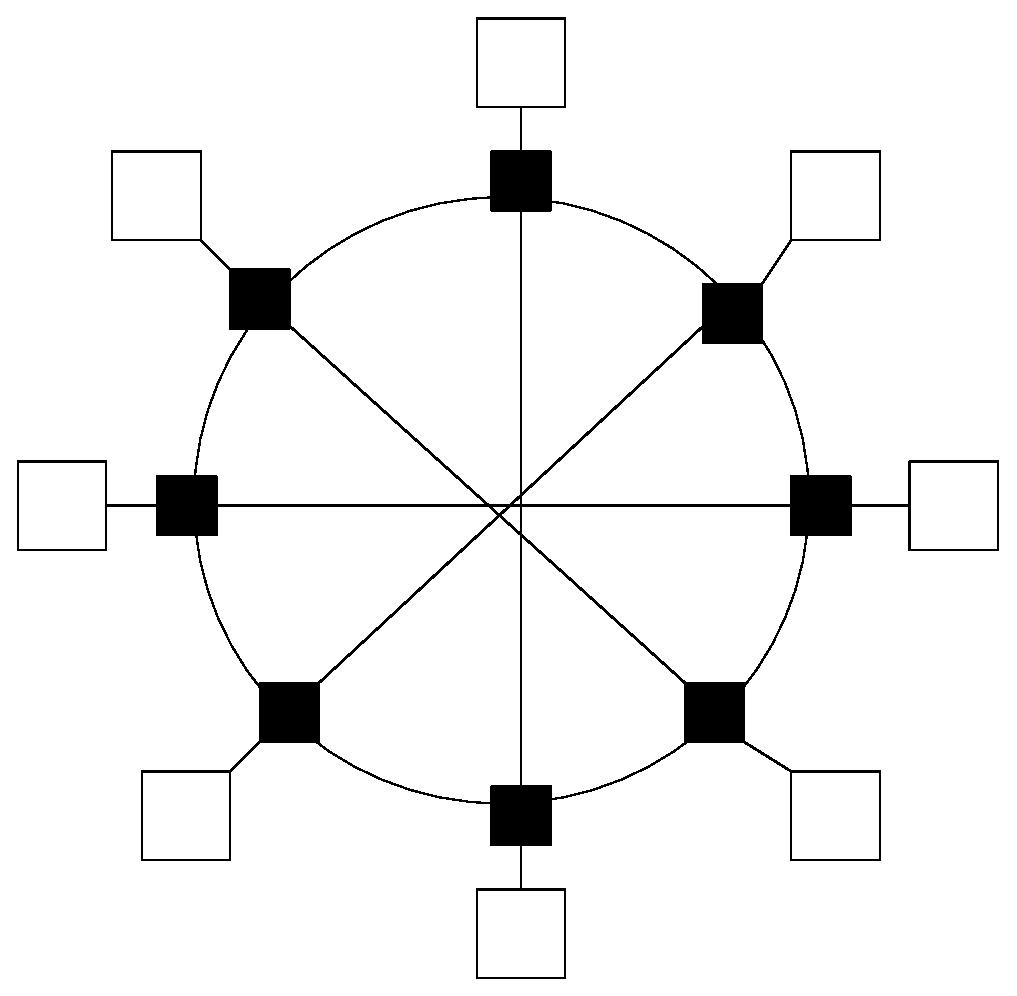
\includegraphics[width=.9\linewidth]{octagon.eps}
  \caption{Octagon}
  \label{fig:2.4b}
\end{subfigure}
\caption[Folded Torus and Octagon]{Network topologies (a). Folded Torus (b). Octagon.}
\label{fig:2.4}
\vspace{10mm}
\end{figure}


Finally, an octagon topology is another example of direct networks. It has 8 nodes and 12 links. Messages transferred between any two nodes need to hop at most two times. Nostrum~\cite{Kumar}, Proteo~\cite{Tortosa}, SOCBUS~\cite{Smit} and Octagon~\cite{Karim} NoC architectures are examples of direct networks.

\subsection{Indirect Networks}

In indirect networks, the NI of each node is connected to an external switch and these switches are connected to other switches using point-to-point links. Crossbar can be stated as one of the simplest indirect networks. In crossbar, each PE is connected to other PEs by traversing a single switch. Researchers have proposed cost efficient partial crossbar networks, that are smaller and more energy efficient with respect to full crossbar networks~\cite{Pasricha2006}. The main drawbacks of a crossbar network is its scalability.

Some examples of multi-stage indirect networks are shown in Fig.~\ref{fig:2.5}. Figure ~\ref{fig:2.5a} is an example of the fat-tree network topology~\cite{Guerrier2000, Leiserson1985}. In a fat-tree topology, all nodes are only connected to the leaves of the tree. As the number of links at the root increases, more bandwidth is allocated on channels with high traffic. 

Figure~\ref{fig:2.5b} illustrates a 2-ary, 3-fly butterfly topology. A butterfly network can be termed as a blocking multi-stage network. It means that when a contention occurs in the network the data may be temporarily dropped or blocked. 

Another type of indirect network topology is Clos. It is an expensive non-blocking network topology because it consists of several full crossbar networks, but, due to its large bandwidth, it can support high performance. 

Benes network is another indirect networks, which requires a controller to rearrange paths in order to establish a connection. Benes is an example of rearrangeable networks. An example of NoC architecture with indirect network topology is SPIN~\cite{Adriahantenaina}


\begin{figure}
\centering
\begin{subfigure}{.5\textwidth}
  \centering
  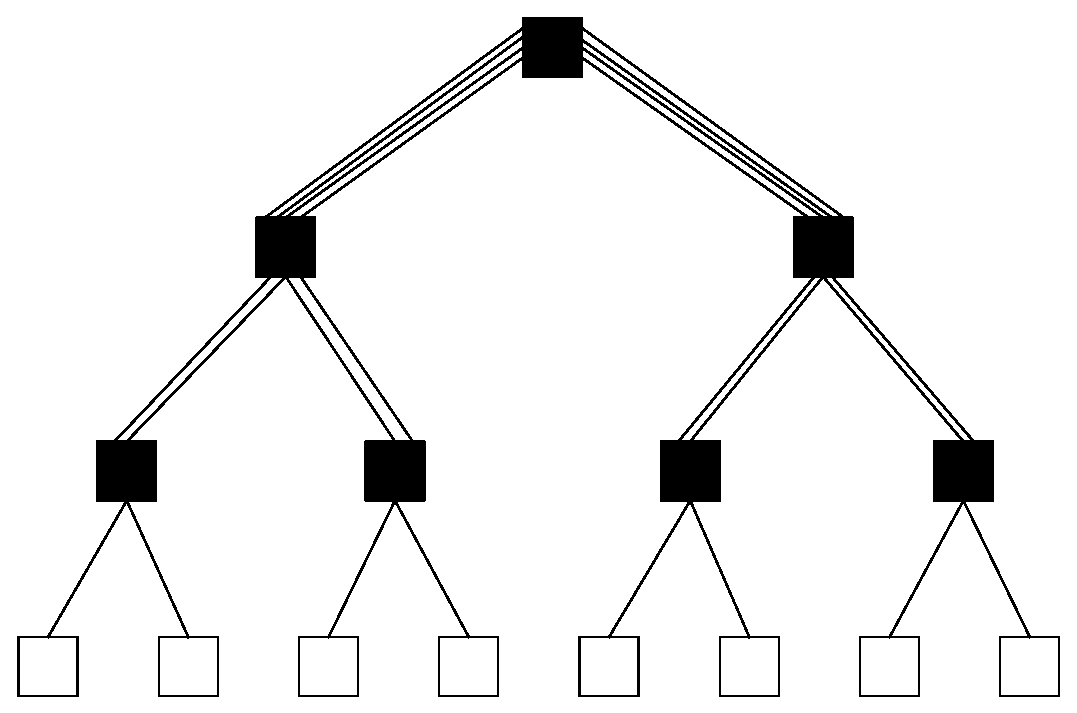
\includegraphics[width=.9\linewidth]{fat_tree.eps}
  \caption{Fat Tree}
  \label{fig:2.5a}
\end{subfigure}%
\begin{subfigure}{.5\textwidth}
  \centering
  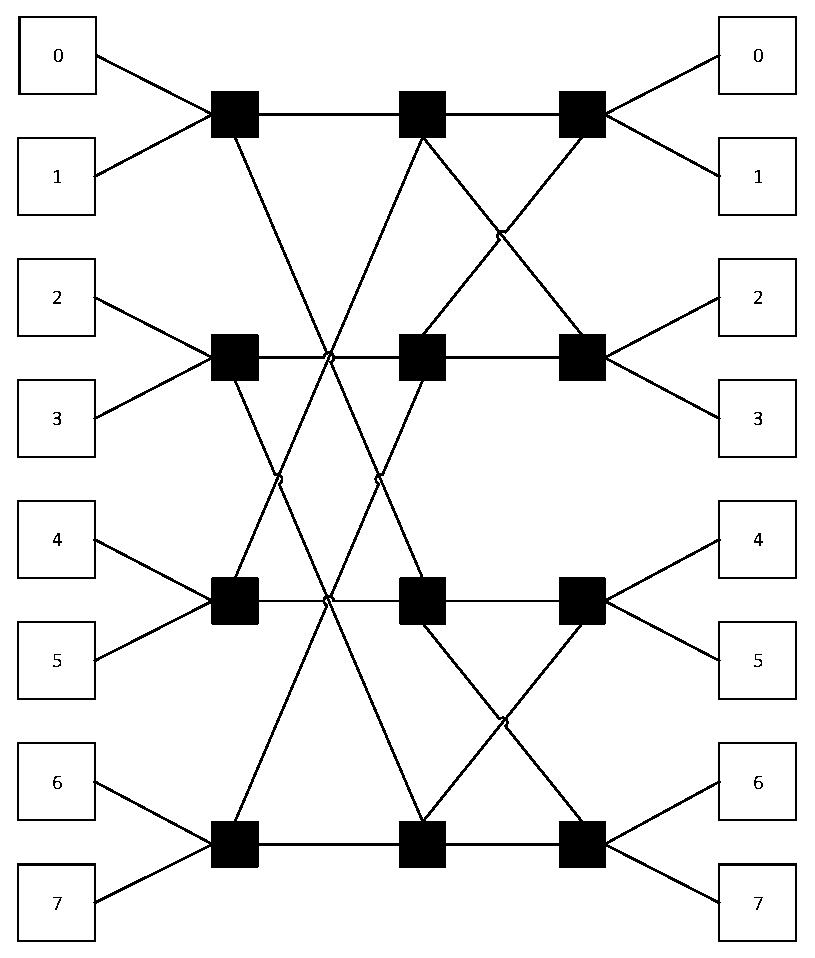
\includegraphics[width=.9\linewidth]{butterfly.eps}
  \caption{Butterfly}
  \label{fig:2.5b}
\end{subfigure}
\caption[Fat Tree and Butterfly]{Network topologies (a). Fat Tree (b). Butterfly.}
\label{fig:2.5}
\vspace{10mm}
\end{figure}


\subsection{Irregular Networks}

Irregular network topologies are also called as ad-hoc networks. These topologies are a mix of direct, indirect and shared bus topologies. The main objectives of this topology are: to reduce the distance between nodes when compared with that of direct and indirect network topologies, and to increase available bandwidth than that of a shared buses. Figure~\ref{fig:2.6a} gives an example of irregular network called optimized (also called as reduced) mesh network which eliminates all unnecessary links and routes. 

There is another kind of irregular network which is named as cluster-based hybrid network. In cluster-based hybrid network, each cluster is a combination of any of the networks (direct, indirect or shared bus based network). Figure~\ref{fig:2.6b} illustrates an example of the cluster-based hybrid network topology which is a combination of ring and mesh network topologies. Examples of NoC architecture which follow irregular topologies are \AE{thereal}~\cite{Goossens} and Xpipes~\cite{Osso}.


\begin{figure}
\vspace{10mm}
\centering
\begin{subfigure}{.5\textwidth}
  \centering
  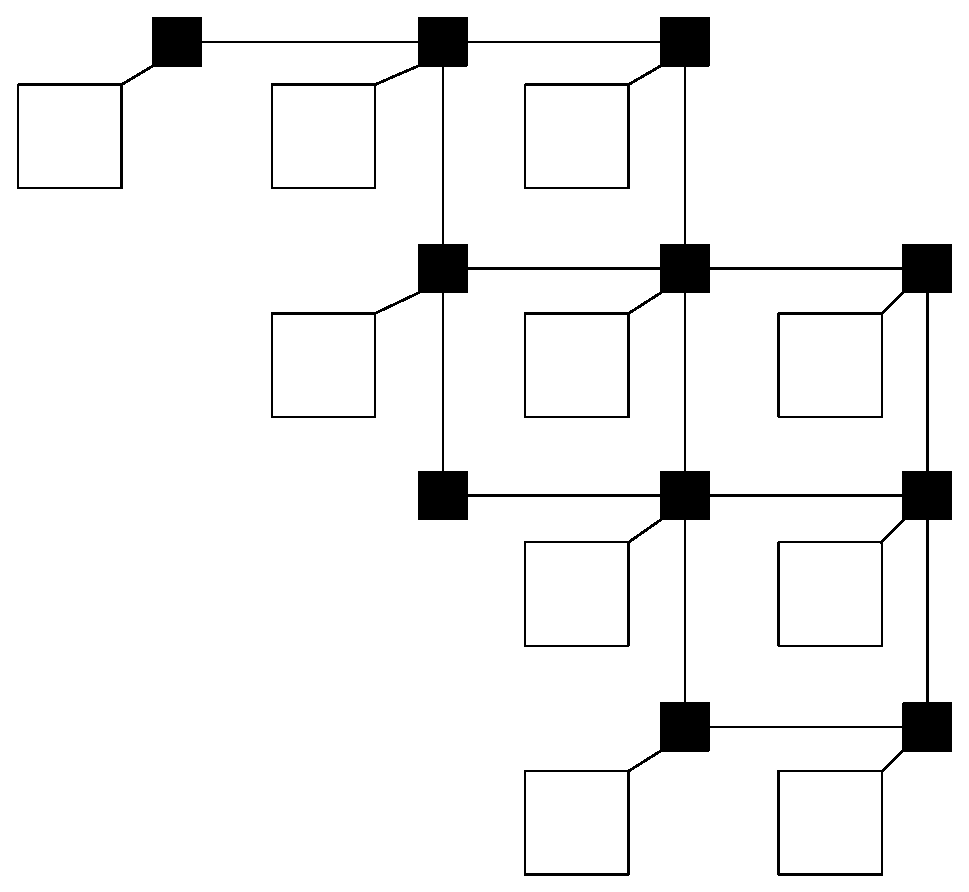
\includegraphics[width=.9\linewidth]{Optimized_mesh.eps}
  \caption{Optimized Mesh}
  \label{fig:2.6a}
\end{subfigure}%
\begin{subfigure}{.5\textwidth}
  \centering
  \includegraphics[width=.9\linewidth]{hybrid.eps}
  \caption{Hybrid}
  \label{fig:2.6b}
\end{subfigure}
\caption[Optimized Mesh and Hybrid]{Network topologies (a). Optimized Mesh (b). Hybrid.}
\label{fig:2.6}
\vspace{10mm}
\end{figure}


\section{Switching Techniques}

The NoC switching technique (strategy) regulates the data flow via routers in the network. Messages sent from PEs (nodes) are split into multiple data \textit{ packets}. A packet is again partitioned into several \textit{flits} (flow control units). A flit is made of one or more \textit{phits} (physical units). A particular NoC architecture has its own message, packet, flit and phit sizes. These affect some factors such as cost, power and performance of NoCs. There are mostly two ways to transport flits in an NoC, they are circuit switching and packet switching. 

\vspace{10mm}
\noindent\textbf{Circuit switching}
\vspace{5mm}

\noindent In circuit switching, a path is reserved between source and destination before starting data transmission. Some routers and links together form a path in the network. When a path (circuit) is reserved, the sender sends a complete message to the receiver. A message header flit travels along the network from source to destination and reserves all the links on its way. If the header flit reaches its destination without encountering any conflict, it sends a positive acknowledgement to the sender. Sender starts data transfer only after receiving positive acknowledgement from header flit. If the path is reserved for any other transmission, header flit sends negative acknowledgement to a sender. The Path is reserved until the completion of data transfer. Circuit switching involves start up waiting time, and also results in low latency data transfer because the bandwidth of the full circuit is reserved for a particular data transfer. The two main virtual circuit switching schemes in use are: allocating one buffer per virtual link and allocating one buffer per link. MANGO~\cite{Bjerregaard} NoC architecture uses variant version of allocating one buffer per virtual link scheme. Nostrum and \AE{thereal} are examples of NoC architectures that use allocating one buffer per link
scheme.

\vspace{0.5cm}
\noindent\textbf{Packet switching}
\vspace{5mm}

\noindent In packet switching, packets are sent from sender to receiver without establishing any path. Packets make their own independent way from source to destination, during the retransmission. Packets follow different routes during the transmission and also have different delays. Packet switching does not have any start up waiting time. The main drawback in packet switching is that it has variable delays during transmission due to the traffic in the network. Several packets arrive at a router and attempts to use the link, only one packet can access the link each time and the other packets should wait for the link to become free. There are three packet switching schemes such as: store and forward, virtual cut through and wormhole switching.


\section{Routing algorithms}
Routing algorithms are necessary to route packets or circuits efficiently from source to destination. Routing schemes are categorized into several groups such as: static or dynamic routing, minimal or non-minimal routing and distributed or source routing.

\vspace{0.5cm}
\noindent\textbf{Static and dynamic routing}
\vspace{5mm}

\noindent NoC router can take decisions which are either static (also named as oblivious or deterministic) or dynamic (also named as adaptive). Static routing uses fixed routes in order to transfer data from source to destination. Static routing does not require any complex router logic, which makes its implementation easier. Routing decisions in static routing are made without considering the traffic at routers and links, and current state of network. Static routing allows the packets to be split among various paths between a source and destination, in a predefined manner. If static routing uses only one path to transfer packets, they are transferred in order. Since the packets reach a target in the order of transmission, there is no need to reorder them at destination, that is no bits are added to packets at NI in order to identify the correct packet sequence. Examples of static routing algorithms are as follows: dimension order routing~\cite{Dally}, XY~\cite{Dehyadgari}, surrounding XY~\cite{Bobda}, pseudo-adaptive XY~\cite{Dehyadgari}, turn model (negative-first, west-first, north-last)~\cite{Kariniemi}, ALOAS~\cite{Kim}, valiant's random~\cite{Dally}, topology adaptive~\cite{Bartic}, source~\cite{Dally2001}, destination tag~\cite{Dally} and random walk routing~\cite{Pirretti}.

Dynamic routing (also called as adaptive) will consider the current state of the network and it is also aware of the load on routers and links when taking routing decisions. Depending on the traffic conditions in the network, the path between a source and destination changes dynamically. In dynamic routing, there is a need for additional resources for monitoring the traffic in the network and to change the routing paths dynamically. However, dynamic routing distributes traffic in a network and make use of alternate paths, when certain paths are congested. Static routing is used when there are predictable traffic conditions in a network, whereas dynamic routing is preferred when traffic in the network is unpredictable and irregular. Examples of dynamic routing algorithms are as follows: minimal adaptive~\cite{Dally}, fully adaptive~\cite{Dally}, congestion look ahead~\cite{Kim2005}, IVAL~\cite{Kariniemi}, odd-even~\cite{Hu}, hot potato~\cite{Feige} and slack time aware routing~\cite{Andreasson}.

\vspace{0.5cm}
\noindent\textbf{Distributed and source routing}
\vspace{5mm}

\noindent Further classification of static and dynamic routing schemes depends on factors such as: where the routing information is saved and where routing decisions are made. In distributed routing, router is responsible for making the routing decisions. In this routing, destination address is carried by the packet. Router either looks up for a destination address or executes a hardware function. Router implements a function whose input is packet's destination address and output is routing decision.

In source routing, each node's (PEs) NI has precomputed routing tables. When a data packet is sent by source node, the router (NI) at the source, reads packet destination address and looks up for the routing information in a table. This routing information is attached to the packets header. When packet reaches any router, the routing information present in the routing header of packet is extracted by router. Source routing does not need any destination address in a packet and also table or functions are not needed to calculate route.

\vspace{10mm}
\noindent\textbf{Minimal and non-minimal routing}
\vspace{5mm}

\noindent Routing schemes are also classified as minimal and non-minimal distance routing. A routing is said to be minimal if the path between the source and destination nodes is of shortest possible length. In minimal routing, source does not send any packets if the shortest path is busy and not available. 

Non-minimal routing does not follow any constraints, instead it uses longer path if the shorter path is not available. This results in many alternative paths, thus helping in avoiding congestion in the network. Drawback with this non-minimal routing is that it consumes more power.










 

